\documentclass[12pt,
bibtotoc,liststotoc,appendixprefix
twoside,paper=a4,headings=small]{scrbook}
%
% Packages
% -----------------------------------
\usepackage[
  paper=a4paper,
  left=12.5mm,
  right=25mm,
  top=25mm,
  bottom=50mm,
  bindingoffset=10mm]{geometry}		% Seitenränder und Bindungskorrektur einstellen
  
\usepackage{apacite} 				% Literatur-Referenzen: American Psycholog. Assoc.
\usepackage{natbib}					

\setcitestyle{round,aysep={}} 		% Indizierg. in runden Klammern, zw. Autor u. Jahr
\usepackage[utf8]{inputenc} 		% Umlaute im Text
\usepackage{ngerman}				% Rechtschreibg.
\usepackage[T1]{fontenc}
\usepackage{lmodern}				% Schriftfamilie
\usepackage{microtype}				% für die Mikrotypografie (besseres Schriftbild)

\usepackage{graphicx} 				% Grafiken einfügen (pdf,png - aber jpg vermeiden)
\graphicspath{{./Bilder/}}          % Pfad zu den Bildern

\usepackage{url}					% URL's formatieren (z.B. in Literatur) 
\usepackage[colorlinks,linkcolor=black,citecolor=black,urlcolor=black]{hyperref} 				% für Hyperlinks in PDF-Dokumenten   
  
\usepackage{tabularx} 				% bessere Gestaltung von Tabellen
\usepackage{longtable} 		
\usepackage{multicol}				
\usepackage{multirow}
\usepackage{booktabs}
\usepackage{tabularx}
		
\usepackage[active]{srcltx}

\usepackage{listings}				% Algorithmen

\usepackage{mdwlist}				% Listen

\usepackage{setspace} 				% Zeileneinstellung
\newtheorem{mydef}{Merksatz}  		% Falls Beispiele, Merksätze m. fortl. Nr. gebr. werden
\newtheorem{bsp}{Beispiel}

\usepackage{todonotes}				% zum Erstellen von ToDos im Editor

\usepackage{lscape}					% zum Rotieren von Seiten

\usepackage{amsmath}				% zum Schreiben von mathematischen Formeln

\usepackage{calc}

\usepackage{footnote}				% Fußnoten
\usepackage{tablefootnote}			% Fußnoten in Tabellen

%\clubpenalty = 10000
%\widowpenalty = 10000 \displaywidowpenalty = 10000

\hyphenation{voll-st\"andigen}		% Worttrennungen global definieren

\setcounter{tocdepth}{1}			% Ebenen, die im Inhaltsverzeichnis angezeigt werden

% Document
% -----------------------------------
\begin{document}

\frontmatter 
    % Titelseite soll keine Kopf oder Fußzeile haben
\thispagestyle{empty}

% Alle Elemente sollen zentriert sein
\begin{center}

\vspace*{-10mm}

\begin{figure}[h]
	\centering
		
\includegraphics[width=0.20\textwidth]{./Bilder/fu_logo.pdf}
\end{figure}

\vspace*{-10mm}

{\LARGE PROFESSUR FÜR \\ANGEWANDTE STATISTIK\\[1mm]}
DER FREIEN UNIVERSITÄT BERLIN\\

\vspace*{3cm}


% Art der Arbeit => (Bachelorarbeit ,Diplomarbeit, Masterarbeit, Seminararbeit)
{\Large \textbf{Seminararbeit}}\\ 

\vspace{1cm}

% Titel der Arbeit 
{\Large \textbf{Topic models}}\\ 
\vspace*{1mm}
{\Large \textbf{applied to song texts}}\\ 
\vspace*{1mm}
% {\Large \textbf{Zeilen verteilt werden wenn nötig}}\\

\vspace{3.5cm}

% Name des/der Autors/Autoren
{\LARGE Silvia Ventoruzzo}\\[15mm]

% Gutachter, Kontaktdaten und Abgabetermin
\parbox{120mm}{
\begin{large}
\begin{tabbing}
Gutachter(in): \hspace{.7cm} \=Prof. Dr. Timo Schmid\\[4mm]
Kurs:\>Seminar zu angewandten Statistik\\
Semester:\> Sommersemester 2019\\
%Verfasser:\> Vorname Nachname\\ % alphabetische Reihenfolge (Nachname)
Matrikel-Nr.:\> 1234567\\
%Adresse:\> Straße Nr, PLZ Ort\\
%Email:\> mail@mail.de\\
%Telefon:\>030-123 456 78\\
[8mm]
\textbf{Abgabetermin:} \> \textbf{01. Januar 2099}\\
\end{tabbing}
\end{large}
}

\end{center}
\clearpage{\pagestyle{empty}\cleardoublepage}
 			% Titelblatt
    \newpage
    \clearpage{\pagestyle{empty}\cleardoublepage}
    \onehalfspacing                  	% Zeilenabstand ab hier 1.5 zeilig
    \tableofcontents 					% Inhaltsverzeichnis
    \clearpage{\pagestyle{empty}\cleardoublepage} 
    
    \listoffigures 					 	% Abbildungsverzeichnis
    \clearpage{\pagestyle{empty}\cleardoublepage}
    
    \listoftables						% Tabellenverzeichnis rein
    \clearpage{\pagestyle{empty}\cleardoublepage}
% -----------------------------------
\mainmatter 							% die einzelnen Kapitel
    \chapter{Einleitung}

Vestibulum fringilla pede sit amet augue. In turpis. Pellentesque posuere. Praesent turpis. Aenean posuere, tortor sed cursus feugiat, nunc augue blandit nunc, eu sollicitudin urna dolor sagittis lacus. Donec elit libero, sodales nec, volutpat a, suscipit non, turpis. Nullam sagittis. Suspendisse pulvinar, augue ac venenatis condimentum, sem libero volutpat nibh, nec pellentesque velit pede quis nunc. Vestibulum ante ipsum primis in faucibus orci luctus et ultrices posuere cubilia Curae; Fusce id purus. Ut varius tincidunt libero. Phasellus dolor. Maecenas vestibulum mollis diam. Pellentesque ut neque. Pellentesque habitant morbi tristique senectus et netus et malesuada fames ac turpis egestas. In dui magna, posuere eget, vestibulum et, tempor auctor, justo. In ac felis quis tortor malesuada pretium. Pellentesque auctor neque nec urna. Proin sapien ipsum, porta a, auctor quis, euismod ut, mi. Aenean viverra rhoncus pede. Pellentesque habitant morbi tristique senectus et netus et malesuada fames ac turpis egestas. Ut non enim eleifend felis pretium feugiat. Vivamus quis mi. Phasellus a est. Phasellus magna. In hac habitasse platea dictumst. Curabitur at lacus ac velit ornare lobortis. Curabitur a felis in nunc fringilla tristique.




\section{Problemumfeld}

Vestibulum fringilla pede sit amet augue. In turpis. Pellentesque posuere. Praesent turpis. Aenean posuere, tortor sed cursus feugiat, nunc augue blandit nunc, eu sollicitudin urna dolor sagittis lacus. Donec elit libero, sodales nec, volutpat a, suscipit non, turpis. Nullam sagittis. Suspendisse pulvinar, augue ac venenatis condimentum, sem libero volutpat nibh, nec pellentesque velit pede quis nunc. Vestibulum ante ipsum primis in faucibus orci luctus et ultrices posuere cubilia Curae; Fusce id purus. Ut varius tincidunt libero. Phasellus dolor. Maecenas vestibulum mollis diam. Pellentesque ut neque. Pellentesque habitant morbi tristique senectus et netus et malesuada fames ac turpis egestas. In dui magna, posuere eget, vestibulum et, tempor auctor, justo. 
\begin{figure}
	\centering
		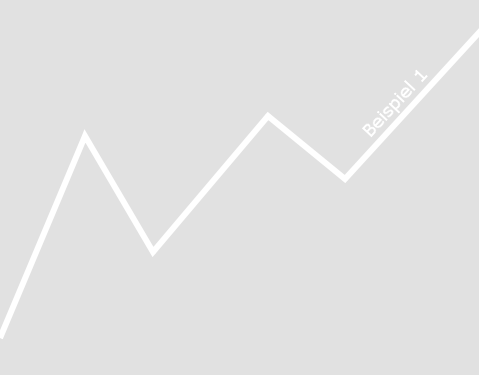
\includegraphics[width=0.7\textwidth]{./Bilder/bsp1.png}
	\caption{Beispiel 1 zum Einfügen einer Grafik}
	\label{fig:bsp1}
\end{figure}

In ac felis quis tortor malesuada pretium. Pellentesque auctor neque nec urna. Proin sapien ipsum, porta a, auctor quis, euismod ut, mi. Aenean viverra rhoncus pede. Pellentesque habitant morbi tristique senectus et netus et malesuada fames ac turpis egestas. Ut non enim eleifend felis pretium feugiat. Vivamus quis mi. Phasellus a est. Phasellus magna. In hac habitasse platea dictumst. Curabitur at lacus ac velit ornare lobortis. Curabitur a felis in nunc fringilla tristique. 

\section{Zielsetzung}

Vestibulum fringilla pede sit amet augue. In turpis. Pellentesque posuere. Praesent turpis. Aenean posuere, tortor sed cursus feugiat, nunc augue blandit nunc, eu sollicitudin urna dolor sagittis lacus. Donec elit libero, sodales nec, volutpat a, suscipit non, turpis. Nullam sagittis. Suspendisse pulvinar, augue ac venenatis condimentum, sem libero volutpat nibh, nec pellentesque velit pede quis nunc. Vestibulum ante ipsum primis in faucibus orci luctus et ultrices posuere cubilia Curae; Fusce id purus. Ut varius tincidunt libero. Phasellus dolor. Maecenas vestibulum mollis diam. Pellentesque ut neque. Pellentesque habitant morbi tristique senectus et netus et malesuada fames ac turpis egestas. In dui magna, posuere eget, vestibulum et, tempor auctor, justo. In ac felis quis tortor malesuada pretium. Pellentesque auctor neque nec urna. Proin sapien ipsum, porta a, auctor quis, euismod ut, mi. Aenean viverra rhoncus pede. Pellentesque habitant morbi tristique senectus et netus et malesuada fames ac turpis egestas. Ut non enim eleifend felis pretium feugiat. Vivamus quis mi. Phasellus a est. Phasellus magna. In hac habitasse platea dictumst. Curabitur at lacus ac velit ornare lobortis. Curabitur a felis in nunc fringilla tristique.

\section{Aufbau der Arbeit}

Vestibulum fringilla pede sit amet augue. In turpis. Pellentesque posuere. Praesent turpis. Aenean posuere, tortor sed cursus feugiat, nunc augue blandit nunc, eu sollicitudin urna dolor sagittis lacus. Donec elit libero, sodales nec, volutpat a, suscipit non, turpis. Nullam sagittis. Suspendisse pulvinar, augue ac venenatis condimentum, sem libero volutpat nibh, nec pellentesque velit pede quis nunc. Vestibulum ante ipsum primis in faucibus orci luctus et ultrices posuere cubilia Curae; Fusce id purus. Ut varius tincidunt libero. Phasellus dolor. Maecenas vestibulum mollis diam. Pellentesque ut neque. Pellentesque habitant morbi tristique senectus et netus et malesuada fames ac turpis egestas. In dui magna, posuere eget, vestibulum et, tempor auctor, justo. In ac felis quis tortor malesuada pretium. Pellentesque auctor neque nec urna. Proin sapien ipsum, porta a, auctor quis, euismod ut, mi. Aenean viverra rhoncus pede. Pellentesque habitant morbi tristique senectus et netus et malesuada fames ac turpis egestas. Ut non enim eleifend felis pretium feugiat. Vivamus quis mi. Phasellus a est. Phasellus magna. In hac habitasse platea dictumst. Curabitur at lacus ac velit ornare lobortis. Curabitur a felis in nunc fringilla tristique. 


    \clearpage{\pagestyle{empty}\cleardoublepage}		% löscht Kopfzeilen und Seitennummerierung von der letzten Seite eines Kapitels, sofern dort kein Text mehr steht
    \chapter{Theory}

Topic models are generative probabilistic models used to ..... [FONTE]. Latent Dirichlet Allocation (LDA) belongs to this category and is specifically a "Bayesian mixture model for discrete data where topics are assumed to be uncorrelated" \citep{hornik2011topicmodels}.

\section{Terminology}
LDA is mainly used in the field of text mining, even though it can be applied to other fields \citep{blei2003latent}. Therefore it is important to firstly explain the RELATIVE terms, as defined by \cite{blei2003latent}:
\begin{itemize}
\item Corpus: a collection of M documents - $D = \{w_1, ..., w_M\}$
\item Document: a sequence of N words - $w = (w_1, ..., w_N)$
\item Word: item from a vocabulary - $w \{1, ..., V\}$
\end{itemize}

It follows that, in looking for the topic distribution for a document in a corpus, one .... following coefficients:
\begin{itemize}
\item $\beta$: term distribution of a topic
\item $\theta$: the proportion of the topic distribution for a document
\end{itemize}


\section{Model definition}
When generating a document $w$ of N words from a $V$-long vocablary from a corpus $D$, LDA follows three steps [FONTE: topicmodels JSS]:
\begin{enumerate}
\item 
\item Document: a sequence of N words - $w = (w_1, ..., w_N)$
\item Word: item from a vocabulary - $w \{1, ..., V\}$
\end{enumerate}

    \chapter{Anwendung}



\section{Daten}



\section{Analyse}


    \clearpage{\pagestyle{empty}\cleardoublepage}
    \chapter{Ergebnisse}

Lorem ipsum dolor sit amet, consectetuer adipiscing elit. Aenean commodo ligula eget dolor. Aenean massa. Cum sociis natoque penatibus et magnis dis parturient montes, nascetur ridiculus mus. Donec quam felis, ultricies nec, pellentesque eu, pretium quis, sem. Nulla consequat massa quis enim. Donec pede justo, fringilla vel, aliquet nec, vulputate eget, arcu. In enim justo, rhoncus ut, imperdiet a, venenatis vitae, justo. Nullam dictum felis eu pede mollis pretium. Integer tincidunt. Cras dapibus. Vivamus elementum semper nisi. Aenean vulputate eleifend tellus. Aenean leo ligula, porttitor eu, consequat vitae, eleifend ac, enim. Aliquam lorem ante, dapibus in, viverra quis, feugiat a, tellus. Phasellus viverra nulla ut metus varius laoreet. Quisque rutrum. Aenean imperdiet. Etiam ultricies nisi vel augue. Curabitur ullamcorper ultricies nisi. Nam eget dui. Etiam rhoncus. Maecenas tempus, tellus eget condimentum rhoncus, sem quam semper libero, sit amet adipiscing sem neque sed ipsum. Nam quam nunc, blandit vel, luctus pulvinar, hendrerit id, lorem. Maecenas nec odio et ante tincidunt tempus. Donec vitae sapien ut libero venenatis faucibus. Nullam quis ante.

\section{Erster Abschnitt}

 Etiam sit amet orci eget eros faucibus tincidunt. Duis leo. Sed fringilla mauris sit amet nibh. Donec sodales sagittis magna. Sed consequat, leo eget bibendum sodales, augue velit cursus nunc, quis gravida magna mi a libero. Fusce vulputate eleifend sapien. Vestibulum purus quam, scelerisque ut, mollis sed, nonummy id, metus. Nullam accumsan lorem in dui. Cras ultricies mi eu turpis hendrerit fringilla. Vestibulum ante ipsum primis in faucibus orci luctus et ultrices posuere cubilia Curae; In ac dui quis mi consectetuer lacinia. Nam pretium turpis et arcu. Duis arcu tortor, suscipit eget, imperdiet nec, imperdiet iaculis, ipsum. Sed aliquam ultrices mauris. Integer ante arcu, accumsan a, consectetuer eget, posuere ut, mauris. Praesent adipiscing. Phasellus ullamcorper ipsum rutrum nunc. Nunc nonummy metus. Vestibulum volutpat pretium libero. Cras id dui. Aenean ut eros et nisl sagittis vestibulum. Nullam nulla eros, ultricies sit amet, nonummy id, imperdiet feugiat, pede. Sed lectus. Donec mollis hendrerit risus. Phasellus nec sem in justo pellentesque facilisis. Etiam imperdiet imperdiet orci. Nunc nec neque. Phasellus leo dolor, tempus non, auctor et, hendrerit quis, nisi. Curabitur ligula sapien, tincidunt non, euismod vitae, posuere imperdiet, leo. Maecenas malesuada. Praesent congue erat at massa. Sed cursus turpis vitae tortor. Donec posuere vulputate arcu. Phasellus accumsan cursus velit. Vestibulum ante ipsum primis in faucibus orci luctus et ultrices posuere cubilia Curae; Sed aliquam, nisi quis porttitor congue, elit erat euismod orci, ac placerat dolor lectus quis orci. Phasellus consectetuer vestibulum elit. Aenean tellus metus, bibendum sed, posuere ac, mattis non, nunc. Vestibulum fringilla pede sit amet augue. In turpis. Pellentesque posuere. Praesent turpis. Aenean posuere, tortor sed cursus feugiat, nunc augue blandit nunc, eu sollicitudin urna dolor sagittis lacus. Donec elit libero, sodales nec, volutpat a, suscipit non, turpis. Nullam sagittis. Suspendisse pulvinar, augue ac venenatis condimentum, sem libero volutpat nibh, nec pellentesque velit pede quis nunc. Vestibulum ante ipsum primis in faucibus orci luctus et ultrices posuere cubilia Curae; Fusce id purus. Ut varius tincidunt libero. Phasellus dolor. Maecenas vestibulum mollis diam. Pellentesque ut neque. Pellentesque habitant morbi tristique senectus et netus et malesuada fames ac turpis egestas. In dui magna, posuere eget, vestibulum et, tempor auctor, justo. In ac felis quis tortor malesuada pretium. Pellentesque auctor neque nec urna. Proin sapien ipsum, porta a, auctor quis, euismod ut, mi. Aenean viverra rhoncus pede. Pellentesque habitant morbi tristique senectus et netus et malesuada fames ac turpis egestas. Ut non enim eleifend felis pretium feugiat. Vivamus quis mi. Phasellus a est. Phasellus magna. In hac habitasse platea dictumst. Curabitur at lacus ac velit ornare lobortis. Curabitur a felis in nunc fringilla tristique. Lorem ipsum dolor sit amet, consectetuer adipiscing elit. Aenean commodo ligula eget dolor. Aenean massa. Cum sociis natoque penatibus et magnis dis parturient montes, nascetur ridiculus mus. Donec quam felis, ultricies nec, pellentesque eu, pretium quis, sem. Nulla consequat massa quis enim. Donec pede justo, fringilla vel, aliquet nec, vulputate eget, arcu. In enim justo, rhoncus ut, imperdiet a, venenatis vitae, justo. Nullam dictum felis eu pede mollis pretium. Integer tincidunt. Cras dapibus. Vivamus elementum semper nisi. Aenean vulputate eleifend tellus. Aenean leo ligula, porttitor eu, consequat vitae, eleifend ac, enim. Aliquam lorem ante, dapibus in, viverra quis, feugiat a, tellus. Phasellus viverra nulla ut metus varius laoreet. Quisque rutrum. Aenean imperdiet. Etiam ultricies nisi vel augue. Curabitur ullamcorper ultricies nisi. Nam eget dui. Etiam rhoncus...

\section{Zweiter Abschnitt}

Maecenas tempus, tellus eget condimentum rhoncus, sem quam semper libero, sit amet adipiscing sem neque sed ipsum. Nam quam nunc, blandit vel, luctus pulvinar, hendrerit id, lorem. Maecenas nec odio et ante tincidunt tempus. Donec vitae sapien ut libero venenatis faucibus. Nullam quis ante. Etiam sit amet orci eget eros faucibus tincidunt. Duis leo. Sed fringilla mauris sit amet nibh. Donec sodales sagittis magna. Sed consequat, leo eget bibendum sodales, augue velit cursus nunc, quis gravida magna mi a libero. Fusce vulputate eleifend sapien. Vestibulum purus quam, scelerisque ut, mollis sed, nonummy id, metus. Nullam accumsan lorem in dui. Cras ultricies mi eu turpis hendrerit fringilla. Vestibulum ante ipsum primis in faucibus orci luctus et ultrices posuere cubilia Curae; In ac dui quis mi consectetuer lacinia. Nam pretium turpis et arcu. Duis arcu tortor, suscipit eget, imperdiet nec, imperdiet iaculis, ipsum. Sed aliquam ultrices mauris. Integer ante arcu, accumsan a, consectetuer eget, posuere ut, mauris. Praesent adipiscing. Phasellus ullamcorper ipsum rutrum nunc. Nunc nonummy metus. Vestibulum volutpat pretium libero. Cras id dui. Aenean ut eros et nisl sagittis vestibulum. Nullam nulla eros, ultricies sit amet, nonummy id, imperdiet feugiat, pede. Sed lectus. Donec mollis hendrerit risus. Phasellus nec sem in justo pellentesque facilisis. Etiam imperdiet imperdiet orci. Nunc nec neque. Phasellus leo dolor, tempus non, auctor et, hendrerit quis, nisi. Curabitur ligula sapien, tincidunt non, euismod vitae, posuere imperdiet, leo. Maecenas malesuada. Praesent congue erat at massa. Sed cursus turpis vitae tortor. Donec posuere vulputate arcu. Phasellus accumsan cursus velit. Vestibulum ante ipsum primis in faucibus orci luctus et ultrices posuere cubilia Curae; Sed aliquam, nisi quis porttitor congue, elit erat euismod orci, ac placerat dolor lectus quis orci. Phasellus consectetuer vestibulum elit. Aenean tellus metus, bibendum sed, posuere ac, mattis non, nunc. Vestibulum fringilla pede sit amet augue. In turpis. Pellentesque posuere. Praesent turpis. Aenean posuere, tortor sed cursus feugiat, nunc augue blandit nunc, eu sollicitudin urna dolor sagittis lacus. Donec elit libero, sodales nec, volutpat a, suscipit non, turpis. Nullam sagittis. Suspendisse pulvinar, augue ac venenatis condimentum, sem libero volutpat nibh, nec pellentesque velit pede quis nunc. Vestibulum ante ipsum primis in faucibus orci luctus et ultrices posuere cubilia Curae; Fusce id purus. Ut varius tincidunt libero. Phasellus dolor. Maecenas vestibulum mollis diam. Pellentesque ut neque. Pellentesque habitant morbi tristique senectus et netus et malesuada fames ac turpis egestas. In dui magna, posuere eget, vestibulum et, tempor auctor, justo. In ac felis quis tortor malesuada pretium. Pellentesque auctor neque nec urna. Proin sapien ipsum, porta a, auctor quis, euismod ut, mi. Aenean viverra rhoncus pede. Pellentesque habitant morbi tristique senectus et netus et malesuada fames ac turpis egestas. Ut non enim eleifend felis pretium feugiat. Vivamus quis mi. Phasellus a est. Phasellus magna. In hac habitasse platea dictumst. Curabitur at lacus ac velit ornare lobortis. Curabitur a felis in nunc fringilla tristique. Lorem ipsum dolor sit amet, consectetuer adipiscing elit. Aenean commodo ligula eget dolor. Aenean massa. Cum sociis natoque penatibus et magnis dis parturient montes, nascetur ridiculus mus. Donec quam felis, ultricies nec, pellentesque eu, pretium quis, sem. Nulla consequat massa quis enim. Donec pede justo, fringilla vel, aliquet nec, vulputate eget, arcu. In enim justo, rhoncus ut, imperdiet a, venenatis vitae, justo. Nullam dictum felis eu pede mollis pretium. Integer tincidunt. Cras dapibus. Vivamus elementum semper nisi. Aenean vulputate eleifend tellus. Aenean leo ligula, porttitor eu, consequat vitae, eleifend ac, enim. Aliquam lorem ante, dapibus in, viverra quis, feugiat a, tellus. Phasellus viverra nulla ut metus varius laoreet. Quisque rutrum. Aenean imperdiet. Etiam ultricies nisi vel augue. Curabitur ullamcorper ultricies nisi. Nam eget dui. Etiam rhoncus. Maecenas tempus, tellus eget condimentum rhoncus, sem quam semper libero, sit amet adipiscing sem neque sed ipsum. Nam quam nunc, blandit vel, luctus pulvinar, hendrerit id, lorem. Maecenas nec odio et ante tincidunt tempus. Donec vitae sapien ut libero venenatis faucibus. Nullam quis ante. Etiam sit amet orci eget eros faucibus tincidunt. Duis leo. Sed fringilla mauris sit amet nibh. Donec sodales sagittis magna. Sed consequat, leo eget bibendum sodales, augue velit cursus nunc, quis gravida magna mi a libero. Fusce vulputate eleifend sapien. Vestibulum purus quam, scelerisque ut, mollis sed, nonummy id, metus. Nullam accumsan lorem in dui. Cras ultricies mi eu turpis hendrerit fringilla. Vestibulum ante ipsum primis in faucibus orci luctus et ultrices posuere cubilia Curae; In ac dui quis mi consectetuer lacinia. Nam pretium turpis et arcu. Duis arcu tortor, suscipit eget, imperdiet nec, imperdiet iaculis, ipsum. Sed aliquam ultrices mauris. Integer ante arcu, accumsan a, consectetuer eget, posuere ut, mauris. Praesent adipiscing. Phasellus ullamcorper ipsum rutrum nunc. Nunc nonummy metus. Vestibulum volutpat pretium libero. Cras id dui. Aenean ut eros et nisl sagittis vestibulum. Nullam nulla eros, ultricies sit amet, nonummy id, imperdiet feugiat, pede. Sed lectus. Donec mollis hendrerit risus. Phasellus nec sem in justo pellentesque facilisis. Etiam imperdiet imperdiet orci. Nunc nec neque. Phasellus leo dolor, tempus non, auctor et, hendrerit quis, nisi. Curabitur ligula sapien, tincidunt non, euismod vitae, posuere imperdiet, leo. Maecenas malesuada. Praesent congue erat at massa. Sed cursus turpis vitae tortor. Donec posuere vulputate arcu. Phasellus accumsan cursus velit. Vestibulum ante ipsum primis in faucibus orci luctus et ultrices posuere cubilia Curae; Sed aliquam, nisi quis porttitor congue, elit erat euismod orci, ac placerat dolor lectus quis orci. Phasellus consectetuer vestibulum elit. Aenean tellus metus, bibendum sed, posuere ac, mattis non, nunc. Vestibulum fringilla pede sit amet augue. In turpis. Pellentesque posuere. Praesent turpis. Aenean posuere, tortor sed cursus feugiat, nunc augue blandit nunc, eu sollicitudin urna dolor sagittis lacus. Donec elit libero, sodales nec, volutpat a, suscipit non, turpis.


\section{Weitere Abschnitte ...}

Nullam sagittis ... 
    \clearpage{\pagestyle{empty}\cleardoublepage}
    \chapter{Fazit und Ausblick}

(...)
    \clearpage{\pagestyle{empty}\cleardoublepage}

% -----------------------------------
\backmatter 
\bibliographystyle{apacite}				% bei natbib in deutsch
\bibliography{./Literatur/quellen}		% Literaturquellen einbinden 
\newpage
\thispagestyle{empty}

\begin{large}

\vspace*{2cm}

\noindent
Hiermit erkläre ich an Eides statt, dass ich die vorliegende Arbeit selbständig
und ohne unerlaubte fremde Hilfe angefertigt, andere als die
angegebenen Quellen und Hilfsmittel nicht benutzt und die den benutzten
Quellen und Hilfsmitteln wörtlich oder inhaltlich entnommenen Stellen als
solche kenntlich gemacht habe.

\vspace{2cm}

\noindent
Berlin, den 16. Februar 2011

\vspace{3cm}

\hspace*{7cm}%
\dotfill\\
\hspace*{8.5cm}%
\textit{(Unterschrift des Verfassers)}

\end{large}
 			% Eidesstattliche Erklärung (nicht bei Seminararb.)

\end{document}